\section{Alternative Konzepte zur Spannungsregelung}
Da zu Beginn des Projektes noch nicht klar war, um welches Modell es sich beim Detroit genau handelt, wurde zu Beginn eine alternative Schaltung untersucht. Beim Besuch des Museums von Hanspeter Setz konnte ein Rauch und Lang begutachtet werden, bei dem wieder eine andere Schaltung verwendet wurde. Auf diese beiden Schaltungen mit ihren Vor- und Nachteilen soll an dieser Stelle kurz eingegangen werden.

\subsection{Detroit Modell 68}
Als zu Beginn des Projektes das Fahrzeug noch nicht besichtigt werden konnte, wurde mit den bereits vorhandenen Informationen nach der Schaltung gesucht. Dabei wurde vor allem eine Schaltung untersucht, die sich jedoch am Ende als die Falsche heraus gestellt hat. Diese Schaltung soll aber trotzdem hier vorgestellt werden, da sie eine alternative Möglichkeit des selben Herstellers darstellt.

Der Detroit Modell 68 besass eine Batterie mit zwei Zwischenabgriffen, sodass insgesamt drei Spannungen zur Verfügung standen. Diese Spannungen wurden für verschiedene Fahrstufen zur Verfügung gestellt. Die Spannung stieg über die Zwischenabgriffe linear an, bis bei der obersten Stufe $84$ V erreicht wurden. Es ist jedoch nicht bekannt, ob die Batterien unterschiedliche Kapazitäten besassen, um die ungleiche Entladung auszugleichen.

Das Funktionsprinzip dieser Schaltung ist bestechend einfach. Steigt doch mit zunehmender Spannung auch die induzierte Spannung, welche für die Geschwindigkeit verantwortlich ist. Auch sind höhere Leistungen bei höheren Stufen möglich (der Strom wird als limitiert angenommen), womit beispielsweise der grössere Luftwiderstand oder das schnellere Bergauffahren ausgeglichen wird. Nachteilig an dieser Schaltung ist auf jeden Fall die Batterie, die je nach Fahrstufe anders und dadurch ungleichmässig entladen wird. Dadurch ist meist nicht die volle Kapazität der Batterien nutzbar. Einzige Ausnahme wäre der Fall, dass die niedrigeren Stufen lediglich zum Anfahren benötigt werden, anschliessend jedoch mit der höchsten Stufe gefahren wird.

Für diese Batterie wurde bereits eine Schaltung angedacht, die es unter Zuhilfenahme von Dioden ermöglicht, sechs gleich grosse Batterien gleichmässig zu entladen. Die Batterien sind dabei entweder zu dritt in Serie (je zwei parallel), zu zweit in Serie (je drei parallel) oder komplett parallel verschaltet. Diese Schaltung ist in Abbildung \ref{fig:68} gezeigt.

\begin{figure}[h!]
	\centering
		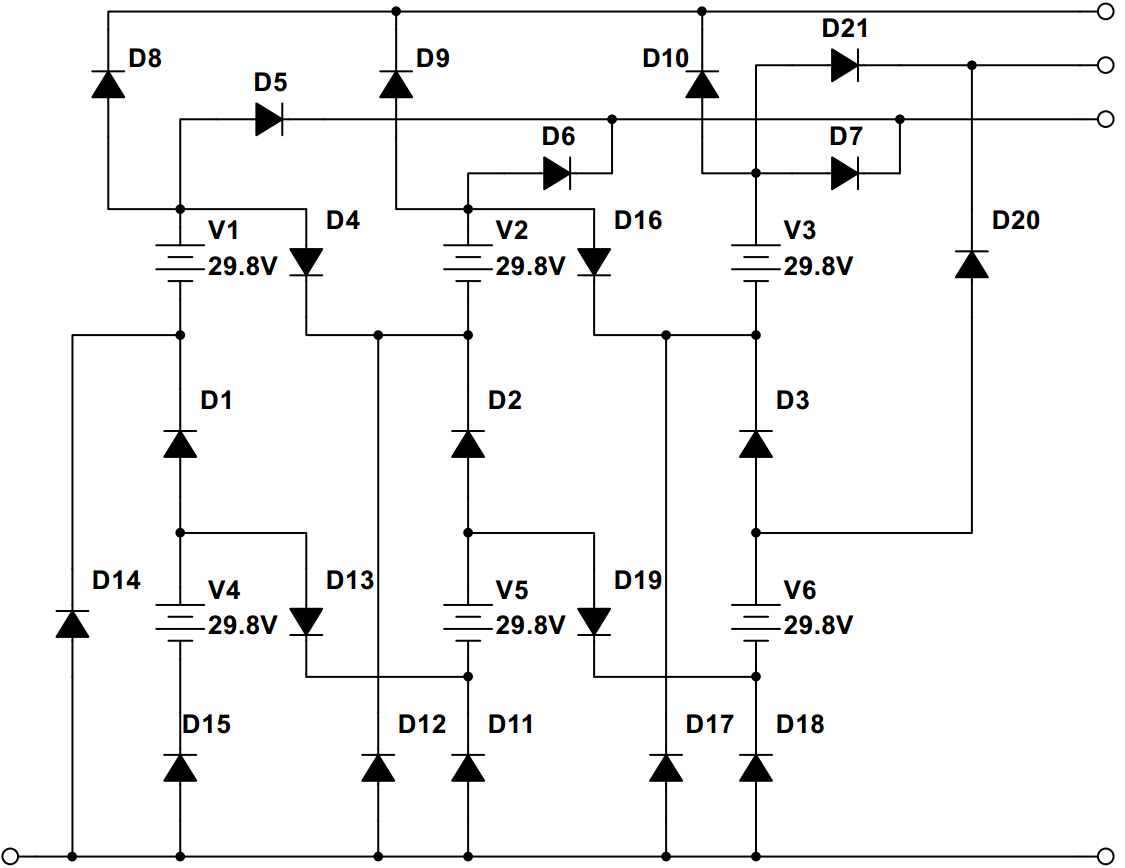
\includegraphics[width=0.65\textwidth]{images/68.PNG}
	\caption{Schaltung für eine Batterie mit Zwischenabgriffen}
	\label{fig:68}
\end{figure}

Mit dieser Schaltung sowie den Batterien des Peugeots wären Spannungen von $0\cdot29.8$ V$=0$ V, $1\cdot29.8$ V$=29.8$ V, $2\cdot29.8$ V$=59.6$ V und $3\cdot29.8$ V$=89.4$ V möglich gewesen, was sehr nahe an den originalen Spannungen gelegen hätte.

\subsection{Rauch und Lang}
Dieses Fahrzeug verfügt über eine sehr einfache Steuerung der Geschwindigkeit. Dazu werden seriell zum Motor verschieden grosse Widerstände hinzugeschaltet, die so die maximal induzierte Spannung im Motor verringern. Auch bei diesem Fahrzeug waren jedoch nur wenige einzelne Fahrstufen vorhanden, wobei der Hebel für jede Stufe ein anderes Plättchen im Schaltkasten herunter drückte, welches den entsprechenden Widerstand mit dem Anker verband. Das Fahrzeug ist in Abbildung \ref{fig:Setz} gezeigt.

\begin{figure}[p]
	\centering
		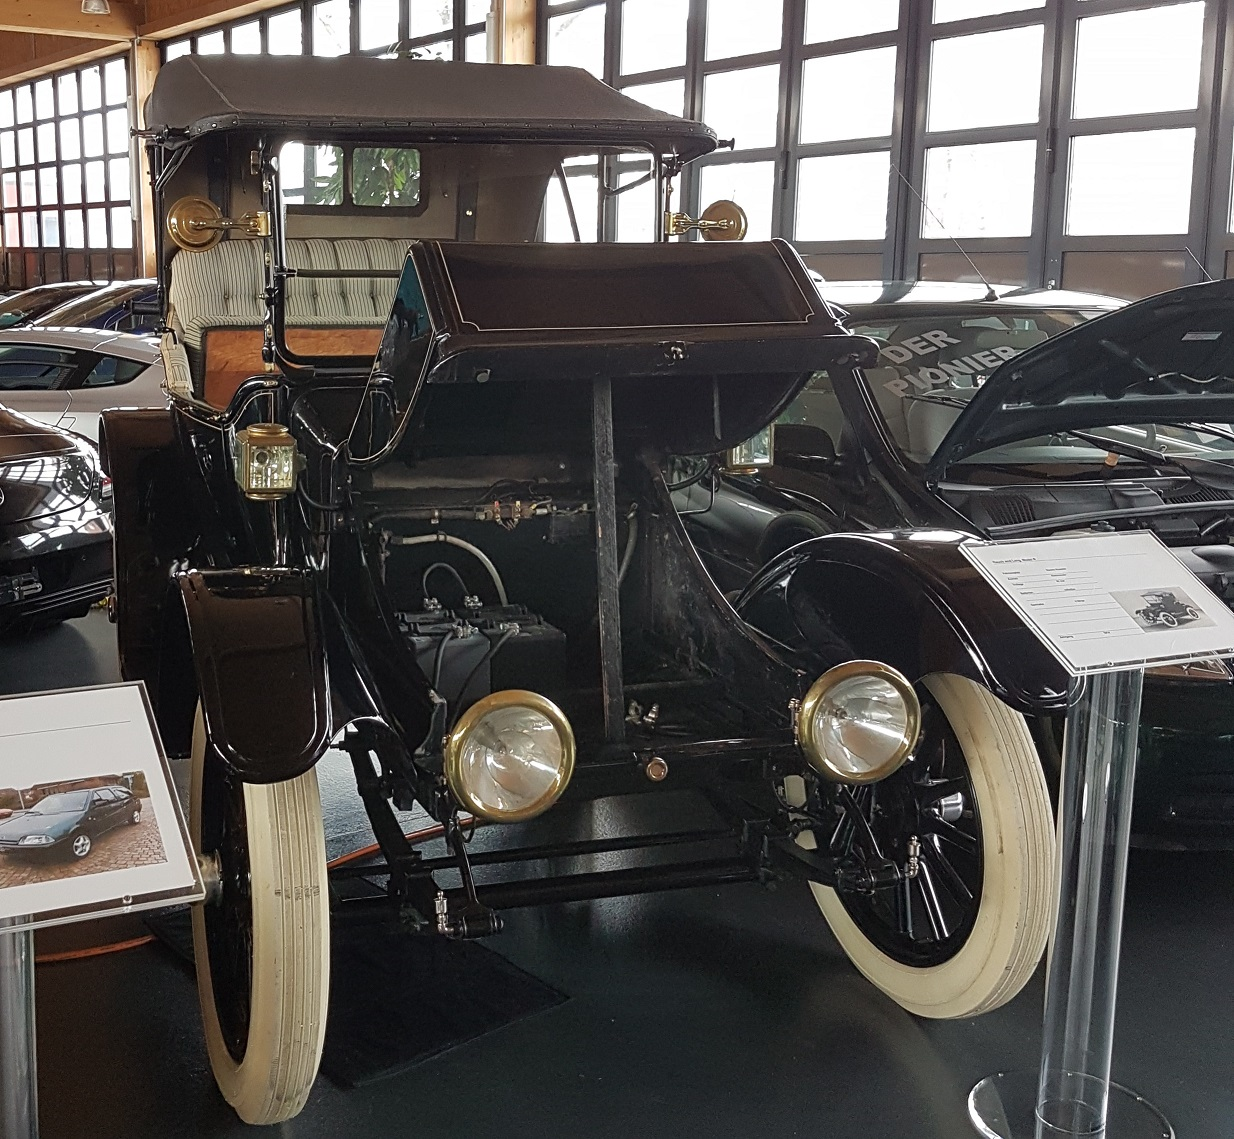
\includegraphics[width=0.8\textwidth]{images/Setz.JPG}
	\caption{Der Rauch und Lang im Museum von Herr Setz}
	\label{fig:Setz}
\end{figure}

Dadurch, dass in beinahe allen Stufen ein zusätzlicher Widerstand zum Motor geschaltet ist, entstehen zusätzliche Verluste im Auto, was die maximale Reichweite reduziert. Auch ist diese Schaltung nicht viel einfacher aufgebaut als die Schaltung des Detroits. Lediglich die Auftrennung auf zwei Batterien entfällt. Anstelle der zusätzlichen Motoranzapfungen für die Feldansteuerungen sind in dieser Schaltung weitere Widerstände nötig. Das Verständnis der Schaltung ist aber bedeutend einfacher: Ein grösserer Widerstand in Serie behindert den Stromfluss zum Motor stärker als ein kleiner Widerstand, sodass dadurch sehr einfach die Leistung reguliert werden kann. Im Gegensatz zur Schaltung des Detroits steigen aber hier das maximale Moment und die erreichbare Geschwindigkeit (bei gegebenem Gegenmoment) mit den höheren Stufen an, da der serielle Widerstand sowohl den maximalen Strom limitiert (beziehungsweise den Stromfluss entsprechend verhindert), als auch die maximal induzierte Spannung bei gegebenem Strom verringert.